\documentclass[tikz,border=1.35mm]{standalone}
\usetikzlibrary{arrows.meta}

\definecolor{externalface}{HTML}{8FB9E8}
\definecolor{splitred}{HTML}{AF2525}
\definecolor{centroidgreen}{HTML}{0E8814}

% Exploded view of face-based isotropic refinement for a hexahedron.
% The eight separated corner cells duplicate shared edge-midpoint, face-centroid,
% and volume-centroid vertices so each child can be read independently.
\begin{document}
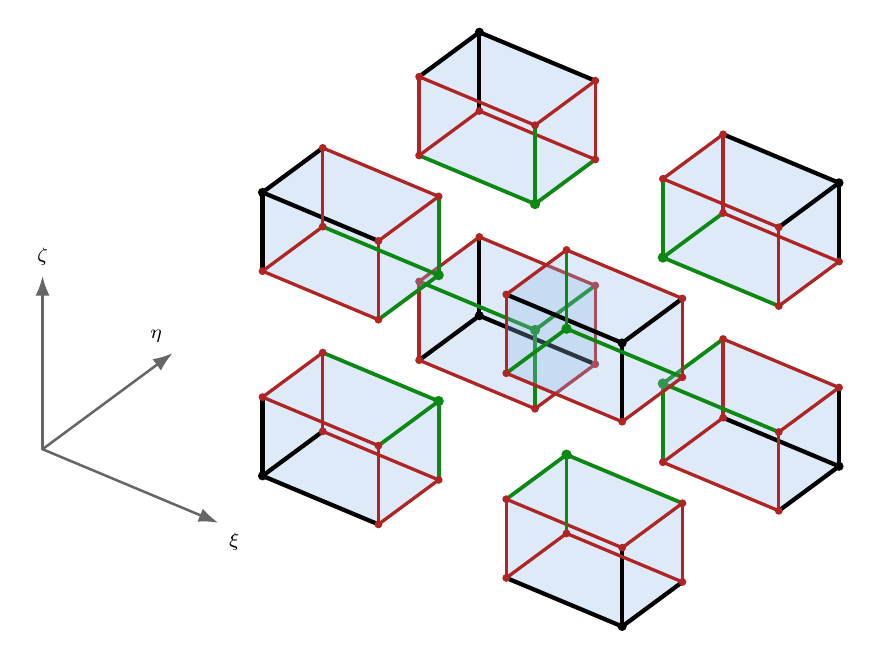
\begin{tikzpicture}[
  x={(20.3mm,-8.5mm)},
  y={(15.3mm,11.3mm)},
  z={(0mm,20mm)},
  line join=round,
  line cap=round,
  outer/.style={draw=black,line width=0.54mm},
  split/.style={draw=splitred,line width=0.42mm},
  centroidedge/.style={draw=centroidgreen,line width=0.48mm},
  cellface/.style={fill=externalface,fill opacity=0.16,draw=none},
  axis/.style={draw=black!60,line width=0.32mm,-{Latex[length=2.5mm,width=1.8mm]}}
]
  \newcommand{\drawcornercell}[8]{%
    \path[cellface] (#1) -- (#2) -- (#5) -- (#3) -- cycle;
    \path[cellface] (#1) -- (#2) -- (#6) -- (#4) -- cycle;
    \path[cellface] (#1) -- (#3) -- (#7) -- (#4) -- cycle;
    \path[cellface] (#2) -- (#5) -- (#8) -- (#6) -- cycle;
    \path[cellface] (#3) -- (#5) -- (#8) -- (#7) -- cycle;
    \path[cellface] (#4) -- (#6) -- (#8) -- (#7) -- cycle;
    \draw[outer] (#1) -- (#2);
    \draw[outer] (#1) -- (#3);
    \draw[outer] (#1) -- (#4);
    \draw[split] (#2) -- (#5);
    \draw[split] (#3) -- (#5);
    \draw[split] (#2) -- (#6);
    \draw[split] (#4) -- (#6);
    \draw[split] (#3) -- (#7);
    \draw[split] (#4) -- (#7);
    \draw[centroidedge] (#5) -- (#8);
    \draw[centroidedge] (#6) -- (#8);
    \draw[centroidedge] (#7) -- (#8);
    \fill[black] (#1) circle[radius=0.58mm];
    \foreach \p in {#2,#3,#4,#5,#6,#7} {
      \fill[splitred] (\p) circle[radius=0.50mm];
    }
    \fill[centroidgreen] (#8) circle[radius=0.66mm];
  }

  % Compact orientation axes, tucked away from the exploded cells.
  \coordinate (Oaxis) at (-1.55,-0.70,-0.55);
  \draw[axis] (Oaxis) -- (-0.45,-0.70,-0.55) node[below right,font=\scriptsize] {$\xi$};
  \draw[axis] (Oaxis) -- (-1.55,0.38,-0.55) node[above left,font=\scriptsize] {$\eta$};
  \draw[axis] (Oaxis) -- (-1.55,-0.70,0.55) node[above,font=\scriptsize] {$\zeta$};

  % Corner A child, shifted away from the parent-cell center.
  \coordinate (AO) at (-0.40,-0.40,-0.40);
  \coordinate (AX) at (0.325,-0.40,-0.40);
  \coordinate (AY) at (-0.40,0.10,-0.40);
  \coordinate (AZ) at (-0.40,-0.40,0.10);
  \coordinate (AXY) at (0.325,0.10,-0.40);
  \coordinate (AXZ) at (0.325,-0.40,0.10);
  \coordinate (AYZ) at (-0.40,0.10,0.10);
  \coordinate (AC) at (0.325,0.10,0.10);

  % Corner B child.
  \coordinate (BO) at (1.85,-0.40,-0.40);
  \coordinate (BX) at (1.125,-0.40,-0.40);
  \coordinate (BY) at (1.85,0.10,-0.40);
  \coordinate (BZ) at (1.85,-0.40,0.10);
  \coordinate (BXY) at (1.125,0.10,-0.40);
  \coordinate (BXZ) at (1.125,-0.40,0.10);
  \coordinate (BYZ) at (1.85,0.10,0.10);
  \coordinate (BC) at (1.125,0.10,0.10);

  % Corner C child.
  \coordinate (CO) at (1.85,1.40,-0.40);
  \coordinate (CX) at (1.125,1.40,-0.40);
  \coordinate (CY) at (1.85,0.90,-0.40);
  \coordinate (CZ) at (1.85,1.40,0.10);
  \coordinate (CXY) at (1.125,0.90,-0.40);
  \coordinate (CXZ) at (1.125,1.40,0.10);
  \coordinate (CYZ) at (1.85,0.90,0.10);
  \coordinate (CC) at (1.125,0.90,0.10);

  % Corner D child.
  \coordinate (DO) at (-0.40,1.40,-0.40);
  \coordinate (DX) at (0.325,1.40,-0.40);
  \coordinate (DY) at (-0.40,0.90,-0.40);
  \coordinate (DZ) at (-0.40,1.40,0.10);
  \coordinate (DXY) at (0.325,0.90,-0.40);
  \coordinate (DXZ) at (0.325,1.40,0.10);
  \coordinate (DYZ) at (-0.40,0.90,0.10);
  \coordinate (DC) at (0.325,0.90,0.10);

  % Corner E child.
  \coordinate (EO) at (-0.40,-0.40,1.40);
  \coordinate (EX) at (0.325,-0.40,1.40);
  \coordinate (EY) at (-0.40,0.10,1.40);
  \coordinate (EZ) at (-0.40,-0.40,0.90);
  \coordinate (EXY) at (0.325,0.10,1.40);
  \coordinate (EXZ) at (0.325,-0.40,0.90);
  \coordinate (EYZ) at (-0.40,0.10,0.90);
  \coordinate (EC) at (0.325,0.10,0.90);

  % Corner F child.
  \coordinate (FO) at (1.85,-0.40,1.40);
  \coordinate (FX) at (1.125,-0.40,1.40);
  \coordinate (FY) at (1.85,0.10,1.40);
  \coordinate (FZ) at (1.85,-0.40,0.90);
  \coordinate (FXY) at (1.125,0.10,1.40);
  \coordinate (FXZ) at (1.125,-0.40,0.90);
  \coordinate (FYZ) at (1.85,0.10,0.90);
  \coordinate (FC) at (1.125,0.10,0.90);

  % Corner G child.
  \coordinate (GO) at (1.85,1.40,1.40);
  \coordinate (GX) at (1.125,1.40,1.40);
  \coordinate (GY) at (1.85,0.90,1.40);
  \coordinate (GZ) at (1.85,1.40,0.90);
  \coordinate (GXY) at (1.125,0.90,1.40);
  \coordinate (GXZ) at (1.125,1.40,0.90);
  \coordinate (GYZ) at (1.85,0.90,0.90);
  \coordinate (GC) at (1.125,0.90,0.90);

  % Corner H child.
  \coordinate (HO) at (-0.40,1.40,1.40);
  \coordinate (HX) at (0.325,1.40,1.40);
  \coordinate (HY) at (-0.40,0.90,1.40);
  \coordinate (HZ) at (-0.40,1.40,0.90);
  \coordinate (HXY) at (0.325,0.90,1.40);
  \coordinate (HXZ) at (0.325,1.40,0.90);
  \coordinate (HYZ) at (-0.40,0.90,0.90);
  \coordinate (HC) at (0.325,0.90,0.90);

  % Draw lower cells first, then upper cells.
  \drawcornercell{AO}{AX}{AY}{AZ}{AXY}{AXZ}{AYZ}{AC}
  \drawcornercell{BO}{BX}{BY}{BZ}{BXY}{BXZ}{BYZ}{BC}
  \drawcornercell{CO}{CX}{CY}{CZ}{CXY}{CXZ}{CYZ}{CC}
  \drawcornercell{DO}{DX}{DY}{DZ}{DXY}{DXZ}{DYZ}{DC}
  \drawcornercell{EO}{EX}{EY}{EZ}{EXY}{EXZ}{EYZ}{EC}
  \drawcornercell{FO}{FX}{FY}{FZ}{FXY}{FXZ}{FYZ}{FC}
  \drawcornercell{GO}{GX}{GY}{GZ}{GXY}{GXZ}{GYZ}{GC}
  \drawcornercell{HO}{HX}{HY}{HZ}{HXY}{HXZ}{HYZ}{HC}
\end{tikzpicture}
\end{document}
